% Slides for 2025-01-13
% To create a slide, use the following:
% \begin{frame}{TITLE}
%     BODY
% \end{frame}

% To create a slide with a bullet list, use the following:
% \begin{frame}{TITLE}
%     \begin{itemize}
%         \item ITEM 1
%         \item ITEM 2
%     \end{itemize}    
% \end{frame}

% To create a slide with numbered list, use the following:
% \begin{frame}{TITLE}
%     \begin{enumerate}
%         \item ITEM 1
%         \item ITEM 2
%     \end{enumerate}
% \end{frame}

% To create a slide with a graphic:
% 1. Add the graphic to this folder (named picture.png)
% 2. Use the following:
% \begin{frame}{TITLE}
%     \centering
%     \includegraphics[height=0.7\textheight,width=0.7\textwidth,keepaspectratio]{picture.png}
% \end{frame}

% To create a slide with two columns, use the following:
% \begin{frame}{TITLE}
%     \begin{columns}
%         \begin{column}{0.5\textwidth}
%             COLUMN 1 BODY
%         \end{column}
%         \begin{column}{0.5\textwidth}
%             COLUMN 2 BODY
%         \end{column}
%     \end{columns}
% \end{frame}

\begin{frame}{Drone System In-place}
    \begin{itemize}
        \item The FDS, Comms Package, and GCS are at MVP or better
        \item Slides will cover diagrams of code
        \item Then demo the frontend + simulator
    \end{itemize}    
\end{frame}

\begin{frame}{FDS Diagram}
    \centering
    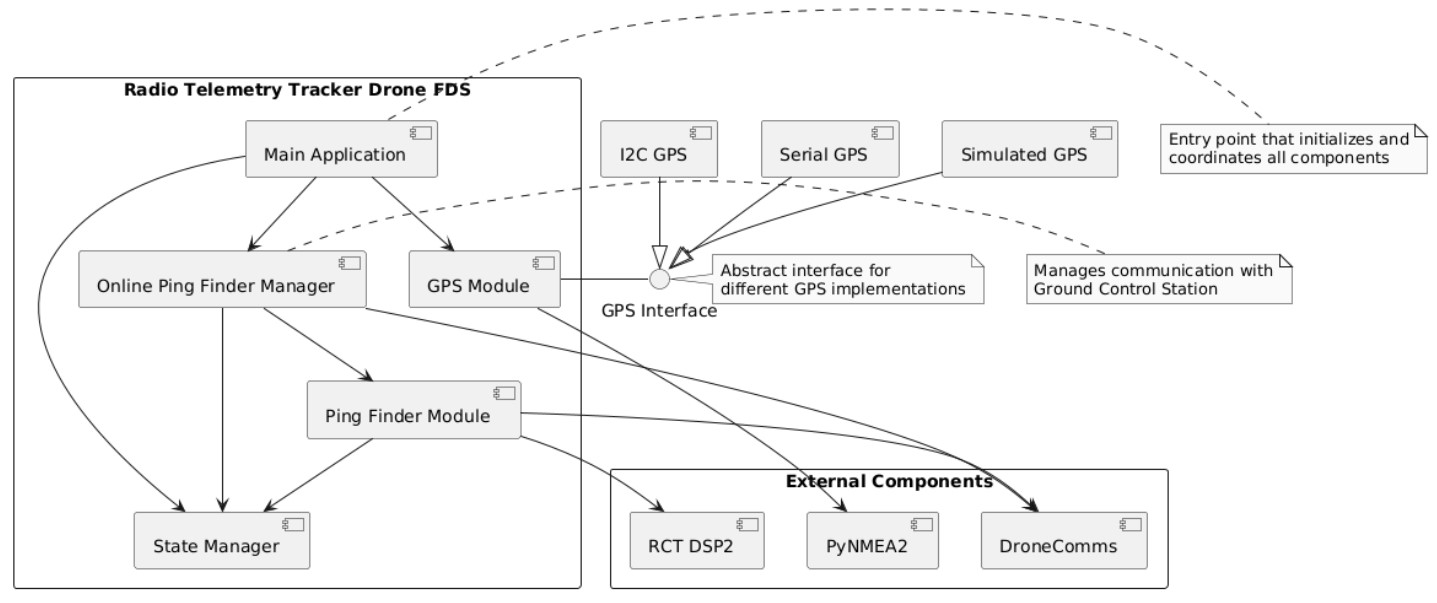
\includegraphics[height=0.7\textheight,width=0.9\textwidth,keepaspectratio]{images/rtt/fds-plantuml.jpg}
\end{frame}

\begin{frame}{Comms Package Diagram}
    \centering
    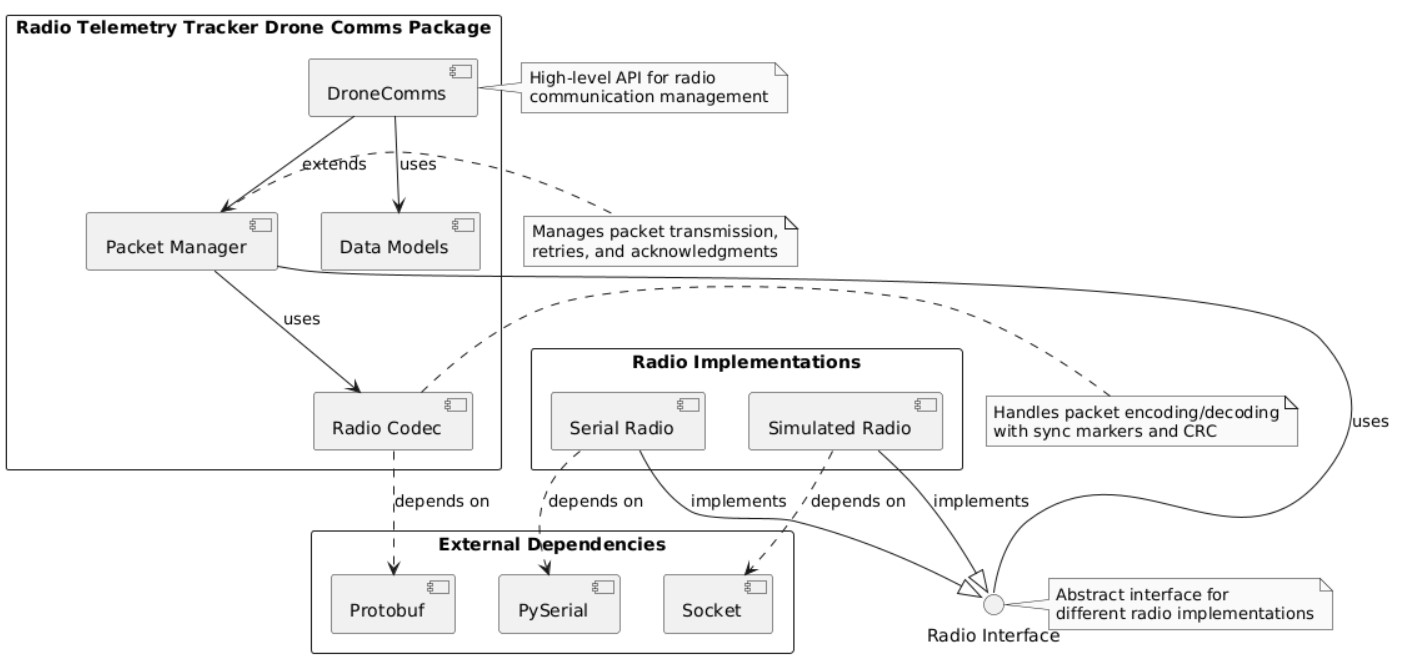
\includegraphics[height=0.9\textheight,width=0.9\textwidth,keepaspectratio]{images/rtt/comms-package-plantuml.jpg}
\end{frame}

\begin{frame}{GCS Diagram}
    \centering
    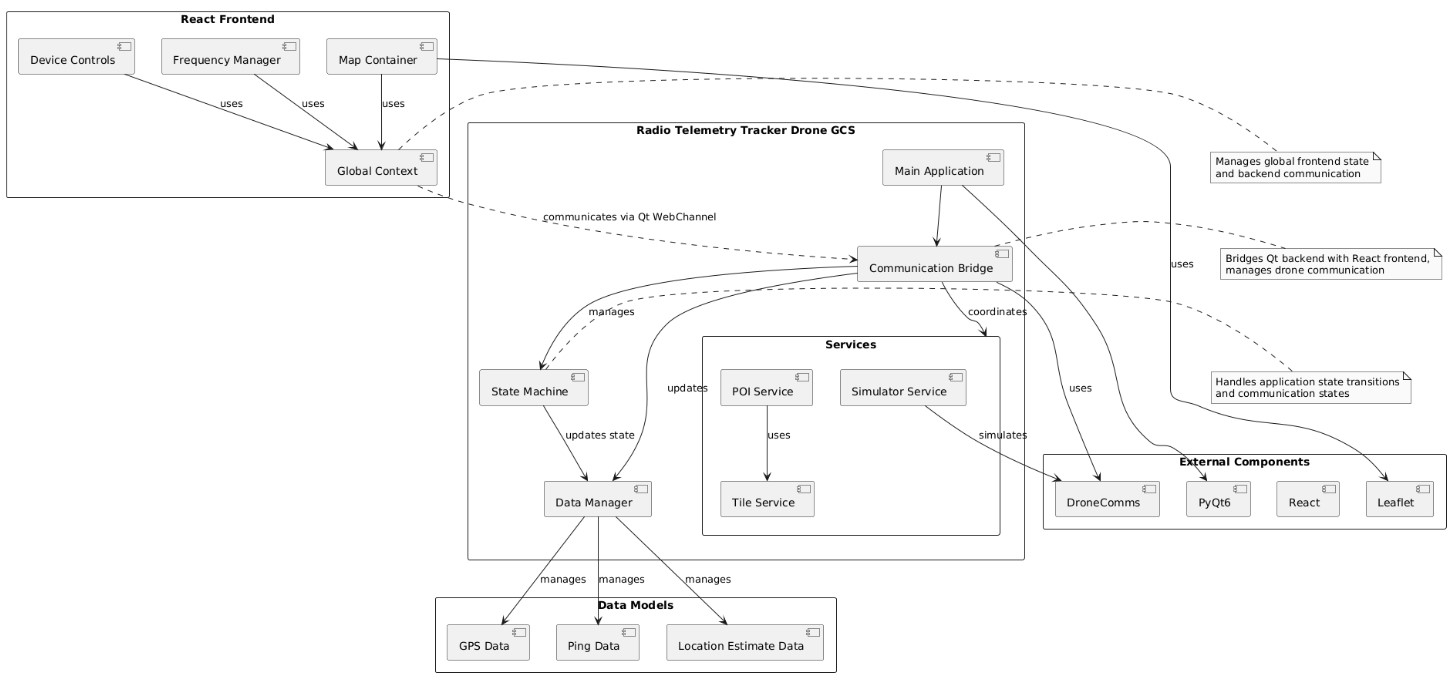
\includegraphics[height=0.9\textheight,width=0.9\textwidth,keepaspectratio]{images/rtt/gcs-plantuml.jpg}
\end{frame}

\begin{frame}{Demo}
    \centering
    Do Demo
\end{frame}

\begin{frame}{Payload Casing}
    \centering
    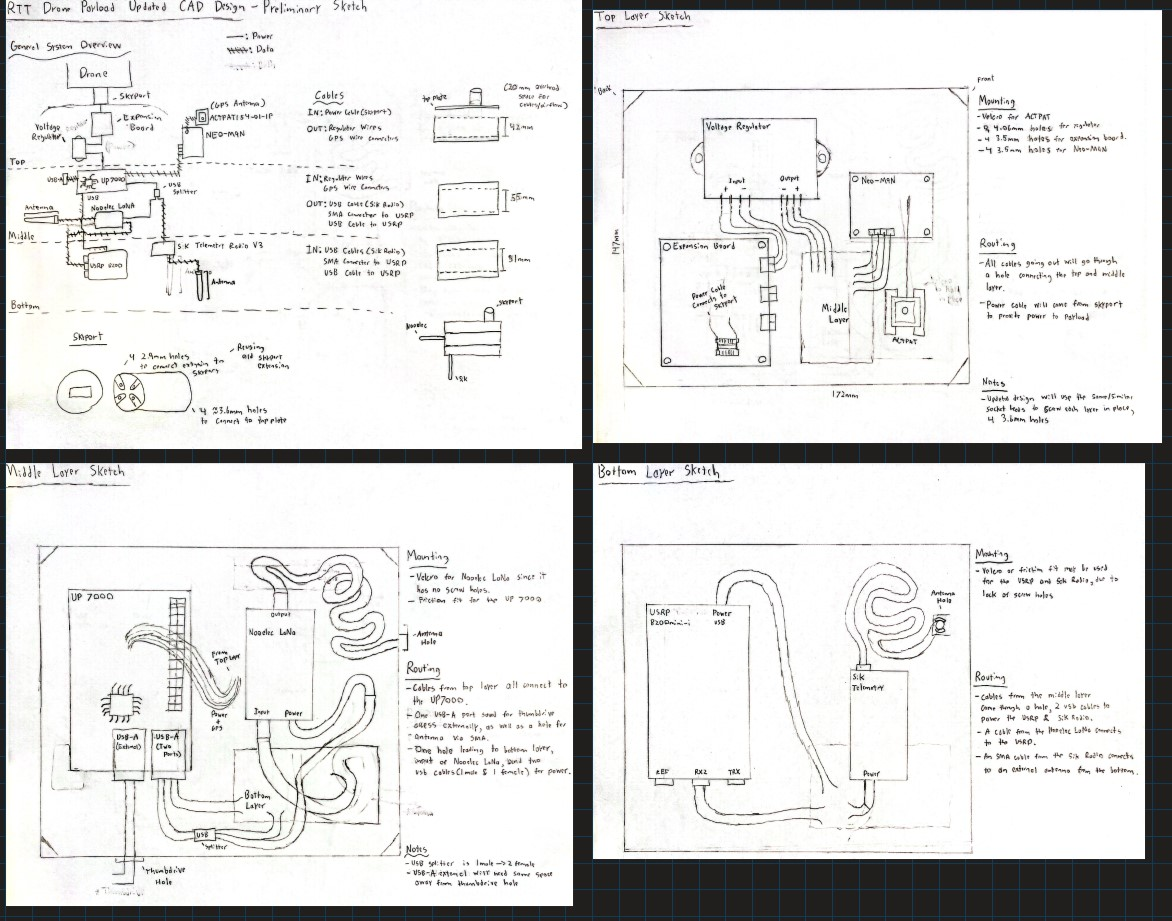
\includegraphics[height=0.7\textheight,width=0.7\textwidth,keepaspectratio]{images/rtt/cad.jpg}
    \begin{itemize}
        \item https://github.com/UCSD-E4E/radio-telemetry-tracker-drone-casing-cad/blob/main/payloadsketch.pdf
    \end{itemize}
\end{frame}


